\documentclass[11pt]{amsart}

 \usepackage{hyperref}
\usepackage{tikz}
\usetikzlibrary{arrows, decorations.markings, decorations.pathmorphing, decorations.pathreplacing, shapes.arrows, patterns, calc}
\usepackage{url}

\tikzset{% arrow close to the source: the 0.2 determines where the arrow is drawn
  ->-/.style={decoration={markings, mark=at position 0.5 with {\arrow{to}}},
              postaction={decorate}},
}

\tikzset{% arrow close to the source: the 0.2 determines where the arrow is drawn
  -<-/.style={decoration={markings, mark=at position 0.5 with {\arrow{to reversed}}},
              postaction={decorate}},
}

\tikzset{% arrow close to the source: the 0.2 determines where the arrow is drawn
  dbl->-/.style={
double, 
double equal sign distance,
shorten >= 1pt,
shorten <= 1pt,
 decoration={markings, mark=at position 0.5 with {\arrow{implies}}},
              postaction={decorate}},
}


\tikzset{% arrow close to the source: the 0.2 determines where the arrow is drawn
  dbl-<-/.style={
double, 
double equal sign distance,
shorten >= 1pt,
shorten <= 1pt,
 decoration={markings, mark=at position 0.5 with {\arrowreversed{implies}}},
              postaction={decorate}},
}






\usepackage{amsmath,amsthm}
\textwidth=14.5cm \oddsidemargin=1cm  \evensidemargin=1cm\setlength{\parskip}{10pt} \setlength{\headsep}{20pt}

\pdfmapfile{+mathpple.map}
\usepackage{mathrsfs}
\usepackage{amscd,amssymb, amsfonts, verbatim,subfigure, enumerate}
\usepackage[mathcal]{eucal}
\usepackage[super]{nth}

\usepackage{mathpazo}



\linespread{1.2}  
\usepackage{color,slashed}



\setcounter{tocdepth}{1}

\renewcommand{\c}{\mf{c}}
\newcommand{\Lap}{\tr}
\newcommand{\dbar}{\br{\partial}}
\newcommand{\Dirac}{\slashed{\partial}}
\newcommand{\RHom}{\mbb{R}\op{Hom}}
\newcommand{\CP}{\mathbb{CP}}
\newcommand{\wbar}{\br{w}} 
\newcommand{\del}{\partial}
\renewcommand{\sl}{\mathfrak{sl}}
\renewcommand{\L}{\mathscr{L}}
\newcommand{\red}[1]{{\color{red}{#1}}} 
\newcommand{\zbar}{\br{z}}
\newcommand{\so}{\mathfrak{so}}
\newcommand{\Spin}{\op{Spin}}
\newcommand{\PV}{\op{PV}}
\newcommand{\GL}{\op{GL}}
\newcommand{\h}{\mathfrak{h}}
\newcommand{\Per}{\mscr{P}}
\newcommand{\dpa}[1]{\frac{\partial}{\partial #1}}
\newcommand{\dpas}[1]{\tfrac{\partial}{\partial #1}}
\newcommand{\Res}{\op{Res}}
\newcommand{\Sup}{\op{Sup}}
\newcommand{\Sing}{\op{Sing}}
\newcommand{\Diag}{\triangle}





\newcommand{\Obs}{\op{Obs}}
\newcommand{\su}{\mathfrak{su}}
\newcommand{\Der}{\op{Der}}

\newcommand{\eps}{\epsilon}
\newcommand{\g}{\mathfrak{g}}

\newcommand{\Hol}{\op{Hol}}

\renewcommand{\Re}{\op{Re}}


\newcommand{\xto}{\xrightarrow}




\newcommand{\what}{\widehat}
\newcommand{\tr}{\triangle}



\newcommand{\til}{\widetilde}
\newcommand{\mscr}{\mathscr}
\renewcommand{\det}{\operatorname{det}}





\newcommand{\br}{\overline}

\newcommand{\iso}{\cong}
\newcommand{\C}{\mathbf C}
\newcommand{\CC}{\mathbf C}
\newcommand{\N}{\mathbf N}
\newcommand{\Q}{\mbf Q}
\newcommand{\rarr}{\rightarrow}
\newcommand{\larr}{\leftarrow}
\newcommand{\norm}[1]{\left\| #1 \right\|}
\newcommand{\Oo}{\mscr O}
\newcommand{\Z}{\mathbb Z}
\newcommand{\defeq}{\overset{\text{def}}{=}}
\newcommand{\into}{\hookrightarrow}


\newcommand{\op}{\operatorname}
\newcommand{\mbf}{\mathbf}
\newcommand{\mbb}{\mathbb}
\newcommand{\mf}{\mathfrak}
\newcommand{\mc}{\mathcal}
\newcommand{\from}{\leftarrow}
\newcommand{\ip}[1]{\left\langle #1 \right\rangle}
\newcommand{\abs}[1]{\left| #1 \right|}

\newcommand{\R}{\mbb R}
\renewcommand{\d}{\mathrm{d}}
\newcommand{\liminv}{ \varprojlim }
\newcommand{\limdir}{\varinjlim}
\newcommand{\dirlim}{\varinjlim}
\newcommand{\fw}{\mathfrak{w}}
\newcommand{\cO}{\mathcal{O}}
\newcommand{\cL}{\mathcal{L}}


\newcommand{\bfP}{\mathbf{P}}


\DeclareMathOperator*{\colim}{colim}
\DeclareMathOperator{\Aut}{Aut} \DeclareMathOperator{\End}{End}

\DeclareMathOperator{\Sym}{Sym} \DeclareMathOperator{\Hom}{Hom}
\DeclareMathOperator{\Spec}{Spec}
\DeclareMathOperator{\Diff}{Diff} 
\DeclareMathOperator{\Met}{Met} \DeclareMathOperator{\Vol}{Vol}
\DeclareMathOperator{\Tr}{Tr}

\def\brian#1{{\textcolor{blue!65!red}{BRW: {#1}}}}
\def\natalie#1{{\textcolor{green!65!black}{BRW: {#1}}}}


%BRIAN STUFF
\newcommand\beqn{\begin{equation}}
\newcommand\eeqn{\end{equation}}









\newtheoremstyle{thm}% name
  {7pt}%      Space above
  {7pt}%      Space below
  {\itshape}%         Body font
  {}%         Indent amount (empty = no indent, \parindent = para indent)
  {\bf}% Thm head font
  {.}%        Punctuation after thm head
  {5pt}%     Space after thm head: " " = normal interword space;
         %       \newline = line-break
  {\thmnumber{#2 }\thmname{#1}\thmnote{ (#3)}}%         Thm head spec (can be left empty, meaning `normal')





\newtheoremstyle{def}% name
  {7pt}%      Space above
  {10pt}%      Space below
  {\itshape}%         Body font
  {}%         Indent amount (empty = no indent, \parindent = para indent)
  {\bf}% Thm head font
  {.}%        Punctuation after thm head
  {5pt}%     Space after thm head: " " = normal interword space;
         %       \newline = line-break
  {\thmnumber{#2} \thmname{#1}\thmnote{ (#3)}}%         Thm head spec (can be left empty, meaning `normal')





\newtheoremstyle{rem}% name
  {4pt}%      Space above
  {10pt}%      Space below
  {}%         Body font
  {}%         Indent amount (empty = no indent, \parindent = para indent)
  {\itshape}% Thm head font
  {:}%        Punctuation after thm head
  {3pt}%     Space after thm head: " " = normal interword space;
        %       \newline = line-break
  {}%         Thm head spec (can be left empty, meaning `normal')

\newtheoremstyle{texttheorem}% name
  {8pt}%      Space above
  {8pt}%      Space below
  {\itshape}%         Body font
  {}%         Indent amount (empty = no indent, \parindent = para indent)
  {\bf}% Thm head font
  {. \hspace{5pt}}%        Punctuation after thm head
  {3pt}%     Space after thm head: " " = normal interword space;
        %       \newline = line-break
  {}%         Thm head spec (can be left empty, meaning `normal')




\theoremstyle{thm}



\newtheorem*{claim}{Claim}
\newtheorem*{theorem*}{Theorem}
\newtheorem*{lemma*}{Lemma}
\newtheorem*{corollary*}{Corollary}
\newtheorem*{proposition*}{Proposition}
\newtheorem*{definition*}{Definition}
\newtheorem{ntheorem}{Theorem}
\newtheorem*{thmA}{Theorem A}
\newtheorem*{thmB}{Theorem B}
\newtheorem*{thmC}{Theorem C}
\newtheorem*{conjecture}{Conjecture}




\newtheorem{theorem}{Theorem}[subsection]
\newtheorem{thm-def}{Theorem/Definition}[theorem]
\newtheorem{proposition}[theorem]{Proposition}
\newtheorem{question}{Question}
\newtheorem*{question*}{Question}
\newtheorem{lemma}[theorem]{Lemma}
\newtheorem{sublemma}[theorem]{Sub-lemma}
\newtheorem{notation}[theorem]{Notation}
\newtheorem{corollary}[theorem]{Corollary}
\newtheorem{deflem}[theorem]{Definition-Lemma}
\newtheorem*{hope}{Hope}
\numberwithin{equation}{subsection}


\theoremstyle{def}
%\theoremstyle{definition}
\newtheorem{definition}[theorem]{Definition}
\newtheorem*{udefinition}{Definition}




\theoremstyle{rem}
%\declaretheorem[style=rem, numbered=no,qed=$\diamondsuit$]{remark}
%\declaretheorem[style=rem, numbered=no,qed=$\diamondsuit$]{remarks}
%\declaretheorem[style=rem, numbered=no,qed=$\diamondsuit$]{example}

\newtheorem*{remark}{Remark}
\newtheorem*{remarks}{Remarks}
\newtheorem*{example}{Example}

%\theoremstyle{texttheorem}
%\newtheorem{textlemma}[theorem]{}

%%This document

\newcommand{\cinfty}{C^{\infty}}



%% BRIAN'S STUFF
\usepackage{cmupint}
\newcommand{\fc}{\mf{c}}






\usepackage{stmaryrd}
\parskip=10pt
\date{}
\newcommand{\gl}{\mf{gl}}





%
\title{Calculations in $\Sym^N T^4$ and $\Sym^N K3$ holography}
%\author{Kevin Costello}
%\author{Natalie M. Paquette}
%\thanks{CALT-TH 2019-050}
%
%\address{Perimeter Institue for Theoretical Physics}
%\address{Walter Burke Institute for Theoretical Physics, California Institute of Technology}
%\email{kcostello@perimeterinstitute.ca}
%\email{nataliep@caltech.edu}


\begin{document}

\maketitle

%After choosing a Calabi--Yau form on $\C^3$, we can write the $\delta$-function along the diagonal in $\C^3 \times \C^3$ as a distributional Dolbeault form
%\[
%\delta_{\Delta} \in \br{\Omega}^{0,3} (\C^3 \times \C^3) .
%\]
%The kernel for the parametrix of the $\dbar$-operator is the distributional Dolbeault form $P'$ satisfying 
%\begin{align*}
%P' & \in \Omega^{0,2} (\C^3 \times \C^3) \\
%\dbar P' & = \delta_{\Delta} .
%\end{align*}
%
%Again using the Calabi--Yau form we can identify 
%\[
%\br\Omega^{0,3}(\C^3 \times \C^3) \cong \br\PV^{3,3}(\C^3 \times \C^3) .
%\]
%We can therefore identify $\delta_{\Delta}$ with a distributational section on the right hand side. 
%Define the so-called `BCOV kernel' by the image of $\delta$-function under the divergence operator
%\[
%\Pi = \del \delta_{\Delta} \in \br\PV^{2,3}(\CC^3 \times \CC^3) .
%\]
%Furthermore, set 
%\[
%P = \del P' \in \br\PV^{2,2}(\CC^3 \times \CC^3) .
%\]

\section{Tree-level OPEs}


Recall that the full classical coupling of Kodaira--Spencer theory is
\[
\int_{\CC^{3|4}} \mu_1 \mu_2 \mu_z \; \d z \d^2 w \d^4 \eta + \int_{\CC^{3|4}} \alpha \mu_i \partial_{w_i} \gamma \; \d z \d^2 w \d^4 \eta + \int_{\CC^{3|4}} \alpha \mu_z \partial_z \gamma \; \d z \d^2 w \d^4 \eta .
\]

Use the notation $D_{r,s}$ for the holomorphic differential operator
\[ 
	D_{r,s} = \frac{1}{r!} \frac{1}{s!} \partial_{w_1}^r \partial_{w_2}^s. 
\]  

\subsection{$\til J \til J$ OPE}

We first compute the OPE of the off-shell operators $\til{J}^i[r,s]$ and then impose constraints to determine the OPE of the on-shell operators $J[r,s]$.

The coefficient of $\til{J}^1[k,l]$ in the OPE will be determined by the terms in the BRST variation of $\mu_1$ which involve $\fc_1$ and $\mu_1$, $\fc_1$ and $\mu_2$, or $\fc_2$ and $\mu_1$. 

Consider the gauge variation of 
\begin{equation}\label{eqn:j1vary}
	\int_{(z,\eta_a) \in \C^{1 \mid 4}} \til{J}^1[r,s](z,\eta_a)  D_{r,s} \mu_1(z,w_i = 0,\eta_a) . 
\end{equation}
The gauge variation of $\mu_1$ is
\begin{align*}
	Q \mu_1 & = \dbar \mf{c}_1 + \mu_i \partial_{w_i} \mf{c}_1 + \mu_z \partial_{z} \mf{c}_1 - \mf{c}_i \partial_{w_i} \mu_1 - \mf{c}_z \partial_z \mu_1 \\
& + \partial_{w_2} \fc_\gamma\partial_z \alpha -  \partial_z\fc_\gamma \partial_{w_2} \alpha + \partial_{w_2} \fc_\alpha \partial_z \gamma - \partial_z \fc_\alpha \partial_{w_2} \gamma .
\end{align*}
For now, we can disregard the terms involving $\fc_\gamma$ and $\alpha$ or $\fc_\alpha$ and $\gamma$.
These will play a role later on when we constrain the OPE's involving the operators $G_\alpha, G_\gamma$.

Inserting this gauge variation into the coupling to $\til{J}^i[r,s]$, we see that the first term, $\dbar \mf{c}_1$, vanishes by integration by parts.  Cancellation of the remaining terms will give us constraints on the OPE coefficients.
The remaining terms are 
\[ 
	\int_{z,\eta_a} \til{J}^1[r,s] (z,\eta_a)  D_{r,s}\left( \mu_i \partial_{w_i} \mf{c}_1 + \mu_z \partial_{z} \mf{c}_1 - \mf{c}_i \partial_{w_i} \mu_1 - \mf{c}_z \partial_z \mu_1 \right)(z,w_i = 0, \eta_a). 
\]
Let us focus on the term in this expression which involves the fields $\mu_1$ and $\mf{c}_1$. This is 
\[ 
	 \int_{z,\eta_a} \til{J}^1[r,s] (z,\eta_a)  D_{r,s}\left( \mu_1 \partial_{w_1} \mf{c}_1   - \mf{c}_1 \partial_{w_1} \mu_1  \right)(z,w_i = 0, \eta_a). 
\]
Because this expression involves both $\mf{c}_1$ and $\mu_1$, which are fields (and a corresponding ghost) that couple to $\til{J}^1$, we find that it can only be cancelled by a gauge variation of an integral involving two copies of the operators $\til{J}^1$, at separate points $z,z'$:  
\[ 
	\tfrac{1}{2} \int_{z,z', \eta_a,\eta_a'} \til{J}^1[k,l] (z,\eta_a) D_{k,l} \mu_1(z, w_i = 0, \eta_a)  \til{J}^1[r,s] (z',\eta'_a) D_{r,s} \mu_1(z', w'_i = 0, \eta'_a) . 
\]
Applying the gauge variation of $\mu_1$ to this expression, and retaining only the terms involving $\dbar \mf{c}_1$, gives us
\[ 
	\int_{z,z', \eta_a,\eta_a'} \til{J}^1[k,l] (z,\eta_a) D_{k,l} \mu_1(z, w_i = 0, \eta_a)  \til{J}^1[r,s] (z',\eta'_a) D_{r,s} \dbar \mf{c}_1 (z', w'_i = 0, \eta'_a) . 
\]
Here the $\dbar$ operator only involves the $z$-component because restricting to $w_i= 0$ sets any $\d \wbar_i$ to zero. We can integrate by parts to move the location of the $\dbar$ operator. Every field $\mu_i$ contains a $\d \zbar$, as otherwise it would restrict to zero at $w_i = 0$, so that $\partial_{\zbar} \mu_i = 0$. 

This discussion shows that in order for the anomaly to cancel we need
\begin{multline} 
	\int_{z,z', \eta_a,\eta_a'} \dbar_{\zbar} \left( \til{J}^1[k,l] (z,\eta_a)  \til{J}^1[r,s] (z',\eta'_a) \right)  D_{m,n} \mu_1(z, w_i = 0, \eta_a)  D_{r,s}  \mf{c}_1 (z', w'_i = 0, \eta'_a)  \\
	= \int_{z'',\eta''_a} \til{J}^1[m,n] (z'',\eta''_a)  D_{m,n}\left( \mu_1 \partial_{w_1} \mf{c}_1   - \mf{c}_1 \partial_{w_1} \mu_1  \right)(z'',w_i = 0, \eta''_a).   
\end{multline}
In these expressions, we sum over the indices $r,s,k,l,m,n$.  This equation must hold for all values of the field $\mu_1$, $\mf{c}_1$. To constrain the OPEs, we can test the equation by setting 
\begin{align*}
\mu_1 & = G(z,\zbar,\eta_a) \d \zbar w_1^k w_2^l \\
\mf{c}_1 & = H(z,\zbar,\eta_a) w_1^r w_2^s
\end{align*}
for $G,H$ arbitrary smooth functions of the variables $z,\zbar,\eta_a$. 

Inserting these values for the fields into the anomaly-cancellation condition gives
\begin{multline} 
	\int_{z,z', \eta_a,\eta_a'} \dbar_{\zbar} \left( \til{J}^1[k,l] (z,\eta_a)  \til{J}^1[r,s] (z',\eta'_a) \right)  G(z,\zbar,\eta_a) H(z',\zbar',\eta_a') \\ 
	= \int_{z'',\eta''_a} (r-k)  \til{J}^1[k+r-1, l+s] (z'',\eta''_a)  G(z'',\zbar'',\eta''_a) H(z'',\zbar'', \eta_a'').
\end{multline}
Since this must hold for all values of the functions $G,H$ we get an identity of the integrands:
\[ 
	\dbar_{\zbar} \left( \til{J}^1[k, l] (z,\eta_a)  \til{J}^1[r,s] (z',\eta'_a) \right)  = \delta_{z = z',\br{z} = \br{z}'} \delta_{\eta_a = \eta'_a} (r-m) \til{J}^1[k + r -1, l+s] .  
\]
(Recall that the fermionic $\delta$-function $\delta_{\eta_a = \eta'_a}$ has the simple expression $\prod_a (\eta_a - \eta'_a)$).  

This in turn leads to the OPE:
\[ 
		\til{J}^1[k,l](0,\eta_a)  \til{J}^1[r,s](z,\eta'_a)  
	\simeq \frac{1}{z} (r-k)  \til{J}^1 [k+r-1,l+s] (0,\eta_a) \delta_{\eta_a = \eta'_a}. 
\]

We apply the fermionic Fourier transform to write this expression in terms of the operators $\til{J}^1[k,l] (0, \what{\eta}^a)$.
We find
\[ 
	\til{J}^1[k,l](0,\what{\eta}^a)  \til{J}^1[r,s](z,\what{\eta}'^{a})  
	\simeq \frac{1}{z} (r-k)  \til{J}^1 [k+r-1,l+s] (0,\what{\eta}^a + \what{\eta}'^{a} ). 
\]

Diagrammatically, the OPE we have just deduced follows from the cancellation of the gauge anomaly in Figure \ref{fig:JJcancel}.


\begin{figure}
	\begin{tikzpicture}
	\begin{scope}
		\node[circle, draw] (J1) at (0,1) {$\til{J}^1$};
		\node[circle, draw] (J2) at (0,-1) {$\til{J}^1$};
		\node (A1) at (2,1)  {$\mu_1$};
		\node (A2) at (2,-1)  {$\mu_1$};
		\draw[decorate, decoration={snake}] (J1) --(A1);
		\draw[decorate, decoration={snake}] (J2) --(A2);
		\draw (0,2) -- (J1) --(J2) -- (0,-2); 
	\end{scope}	
	\begin{scope}[shift={(4,0)}];
		\node[circle, draw] (J) at (0,0) {$\til{J}^1$};
		\node (A1) at (3,1)  {$\mu_1$};
		\node (A2) at (3,-1)  {$\mu_1$};
		\node[circle,draw,fill=black, minimum size = 0.2pt]  (V) at (1.5,0) {};  
		\draw[decorate, decoration={snake}] (J) -- (1.5,0) --  (A1);
		\draw[decorate, decoration={snake}] (1.5,0) --(A2);
		\draw (0,2) -- (J)-- (0,-2);
	\end{scope}
	\end{tikzpicture}
	\caption{Cancellation of the gauge anomaly of these two diagrams leads to the equation for the self OPE of the currents $\til{J}^1[k,l]$. \label{fig:JJcancel}}
\end{figure}

\subsubsection{}

Similarly, we have the $\til{J}^2 \til{J}^2$ OPE
\[ 
		\til{J}^2[r,s](0,\what{\eta}^a)  \til{J}^2[k,l](z,\what{\eta}'^{a})  
	\simeq \frac{1}{z} (l-s)  \til{J}^2 [r+k,s+l-1] (0,\what{\eta}^a + \what{\eta}'^{a} ). 
\]

the $\til{J}^1 \til{J}^2$ OPE
\[ 
	\til{J}^1[r,s] (0,\what{\eta}^a) \til{J}^2[k,l](z,\what{\eta}'^{a}) \simeq - \frac{1}{z} s  \til{J}^1[r+k, l+s - 1] (0,\what{\eta}^a + \what{\eta}'^{a})    + \frac{1}{z} k \til{J}^2[k+r-1,l+s] (0,\what{\eta}^a + \what{\eta}'^{a})  
\]
and the $\til{J}^2 \til{J}^1$ OPE
\[ 
	\til{J}^2[r,s] (0,\what{\eta}^a) \til{J}^1[k,l](z,\what{\eta}'^{a}) \simeq - \frac{1}{z} r  \til{J}^2[r+k-1, l+s ] (0,\what{\eta}^a + \what{\eta}'^{a})    + \frac{1}{z} l \til{J}^1[k+r,l+s-1] (0,\what{\eta}^a + \what{\eta}'^{a}).   
\]

\subsubsection{}

Let us use the these calculations to calculate the OPEs of the on-shell operators 
\[ 
	 	J[r,s] = r \til{J}^2[r-1,s] - s \til{J}^1[r,s-1]. 
\]
We find
\begin{multline}
	J[r,s] (0,\what{\eta}^a) J[k,l](z,\what{\eta}'^{a}) =   \frac{1}{z} (l-s) k r  \til{J}^2 [k+r-2,l+s-1]   \\
	+ \frac{1}{z} ls(k-r) \til{J}^1[k+r-1, l+s-2] \\
	+  \frac{1}{z} r (r-1) l  \til{J}^2[r+k-2, l+s -1 ]    - \frac{1}{z} l (l-1) r \til{J}^1[k+r-1,l+s-2]  \\
	+ \frac{1}{z} k s(s-1)  \til{J}^1[r+k-1, l+s - 2]    - \frac{1}{z}k s  (k-1) \til{J}^2[k+r-2,l+s-1] 
\end{multline}
(On the right hand side, all operators are evaluated at $z = 0$ and with the fermionic variables $\what{\eta}^a+\what{\eta}'^{a}$.  We have dropped this dependence for clarity.)

Collecting the terms, we find the OPE is
\begin{align*} 
	&\frac{1}{z} \left( (l-s)kr + r (r-1) l - ks (k-1)     \right)  \til{J}^2 [k+r - 2, l +s - 1]  \\
	&+ \frac{1}{z} \left( ls (k-r) - l (l-1) r + k s (s-1)  \right) \til{J}^1 [ k + r -1, l + s - 2]. 
\end{align*}

Since 
\[ 
	 J[k+r-1,l+s-1] = (k+r-1)\til{J}^2 [k+r-2,l+s-1] - (l+s-1) \til{J}^1 [ k+r - 1, l +s - 2] 
\]
we find that the OPE is 
\[ 
	J[r,s](0,\what{\eta}^a)J[k,l](z,\what{\eta}'^{a}) = \frac{1}{z} (rl-ks)  J[r+k-1,l+s-1](z, \what{\eta}^a + \what{\eta}'^{a}).     
\]

Note that the operators with $r + s = 2$ which are independent of $\what{\eta}^a$ satisfy the OPE of the $\mf{su}(2)$ Kac-Moody algebra at level \underline{zero}.
We will get a nontrivial level once we include the contribution from the back reaction, which we do in \S \ref{sec:br}. 

As was pointed out in \cite{CP}, the mode algebra corresponding to this full collection of OPE's can be expressed as the super loop space of the Lie algebra $\fw_{\infty}$ of Hamiltonoian vector fields on $\C^2$.\footnote{This is the quotient of the Lie algebra of functions on $\C^2$, which equipped with the standard Poisson bracket, by its center consisting of the constant functions.}
This is the Lie algebra $\cL^{1|4} \fw_\infty$.
Explicitly, elements of this super Lie algebra can be expressed as 
\beqn
z^{n} f(w_1,w_2; \eta_a) \in \cL^{1|4} \fw_\infty
\eeqn
for $n \in \Z$ and where $f(w_1,w_2;\eta_a) \in \C[w_1,w_2,\eta_a]/ \C$. 
The bracket is 
\beqn
[z^n f, z^m g] = z^{n+m} \eps^{ij} \del_{w_i} f \del_{w_j}g .
\eeqn

\subsection{$TJ$ OPE}

We turn to the tree-level OPE between the on-shell operators $T$ and $J$. 
First, we compute the tree-level OPE between the off-shell operators $\til{J}$ and $\til{T}$. 

The coefficient of $\til{J}^1$, for instance, in this OPE will be determined by the terms in the BRST variation of $\mu_1$ which involve $\fc_1$ and $\mu_z$ or $\fc_z$ and $\mu_1$. 
We collect such terms in the gauge variation of \eqref{eqn:j1vary} and 
\begin{equation}\label{eqn:Tvary}
\int_{(z,\eta_a) \in \CC^{1|4}} \til{T} [m,n] (z,\eta_a) D_{m,n} \mu_z(z, w_i=0, \eta_a) .
\end{equation}
Recall that the gauge variation of $\mu_z$ is
\begin{align*}
Q \mu_z & = \dbar \fc_z + \mu_i \partial_{w_i} \fc_z + \mu_z \partial \fc_z - \fc_i \partial_{w_i} \mu_z - \fc_z \partial_z \mu_z \\
& -\epsilon_{ij} \partial_i \fc_\gamma \partial_j \alpha - \epsilon_{ij} \partial_i \fc_\alpha \partial_j \gamma .
\end{align*}
For now, we can disregard the terms involving $\alpha$ and $\fc_\gamma$ or $\fc_\alpha$ and $\gamma$.

The terms in the variations of \eqref{eqn:j1vary} and \eqref{eqn:Tvary} involving $\fc_1$ and $\mu_z$ or $\fc_z$ and $\mu_1$ is
\begin{align*}
& \int_{z, \eta} \til{J}^1[m,n](z,\eta_a) D_{m,n} (\mu_z \partial_{z} \fc_1 - \fc_z \partial_z \mu_1) (z, w_i=0,\eta_a) \\
+ & \int_{z,\eta} \til{T} [m,n](z,\eta_a) D_{m,n}(\mu_1 \partial_{w_1} \fc_z - \fc_1 \partial_{w_1} \mu_z) (z, w_i=0, \eta_a).
\end{align*}
The coefficient of $\fc_z$ can only be cancelled by a gauge variation of 
\[
\int_{z,z',\eta_a,\eta_a'} \til{J}^1 [r,s] (z,\eta_a) D_{r,s} \mu_1(z,w_i=0,\eta_a) \til{T} [k,l] (z',\eta_a') D_{k,l} \mu_z(z',w_i'=0,\eta_a') .
\]
By similar manipulation as above, we find that the gauge variation of this expression is 
\begin{align*}
& \int_{z,z',\eta_a,\eta_a'} \dbar_{z} \left(\til{J}^1 [r,s] (z,\eta_a) \til{T}[k,l](z',\eta_a')\right) D_{r,s} \fc_1 (z,w_i=0,\eta_a) D_{k,l} \mu_z (z',w'_i=0,\eta_a') \\
+ & \int_{z,z',\eta_a,\eta_a'} \dbar_{z'} \left(\til{J}^1 [r,s] (z,\eta_a) \til{T}[k,l](z',\eta_a')\right) D_{r,s} \mu_1 (z,w_i=0,\eta_a) D_{k,l} \fc_z (z',w'_i=0,\eta_a').
\end{align*}

To constrain the OPEs, we use the test functions $\mu_z = 0$, $\fc_1 = 0$, $\mu_1 = G(z,\zbar,\eta_a) \d \zbar w_1^k w_2^l$, 
$\fc_z = H(z,\zbar,\eta_a) w_1^r w_2^s$
for $G,H$ arbitrary smooth functions of the variables $z,\zbar,\eta_a$.
This yields the anomaly cancellation condition
\begin{multline}
\int_{z,z',\eta_a,\eta_a'} \dbar_{z'}\left(\til{J}^1 [r,s] (z,\eta_a) \til{T}[k,l](z',\eta_a')\right) G(z,\zbar,\eta_a) H(z',\zbar', \eta_a') = \\
- \int_{z'', \eta_a''} \til{J}^1[r+k, s+l] (z'', \eta_a'') H(z'', \zbar'', \eta_a'') \partial_{z''} G(z'', \zbar'', \eta_a'') \\ 
+ r \int_{z'',\eta_a''} \til{T}[r+k-1, s+l] (z'',\eta_a'') G(z'',\zbar'', \eta_a'') H(z'',\zbar'', \eta_a'') .
\end{multline}
Integrating the right hand side by parts gives us
\begin{multline}
\int_{z'', \eta_a''} \partial_{z''} \til{J}^1[r+k, s+l] (z'', \eta_a'') H(z'', \zbar'', \eta_a'') G(z'', \zbar'', \eta_a'') \\ +  \int_{z'', \eta_a''} \til{J}^1[r+k, s+l] (z'', \eta_a'') \partial_{z''} H(z'', \zbar'', \eta_a'')  G(z'', \zbar'', \eta_a'') \\
+ r \int_{z'',\eta_a''} \til{T}[r+k-1, s+l] (z'',\eta_a'') G(z'',\zbar'', \eta_a'') H(z'',\zbar'', \eta_a'') 
\end{multline}

Because $G,H$ are arbitrary functions, we arrive at the OPE
\begin{multline}
\til{T}[r,s](0,\eta_a) \til{J}^1[k,l] (z,\eta_a') \simeq \delta_{\eta_a=\eta_a'} \frac1z \partial_z \til{J}^1[r+k,s+l](0,\eta_a) + \delta_{\eta_a=\eta_a'} \frac{1}{z^2} \til{J}^1[r+k,s+l](0,\eta_a) \\ + r \delta_{\eta_a=\eta_a'} \til{T}[r+k-1,s+l] (0,\eta_a).
\end{multline}
Switching the $\eta_a$ variables to $\what{\eta}^a$ variables by applying the odd Fourier transform we can write this OPE as
\begin{multline}
\til{T}[r,s](0,\what{\eta}^a) \til{J}^1[k,l] (z,\what{\eta}'^a) \simeq \frac1z \partial_z \til{J}^1[r+k,s+l](0,\what{\eta}^a + \what{\eta}'^a) + \frac{1}{z^2} \til{J}^1[r+k,s+l](0,\what{\eta}^a + \what{\eta}'^a)  \\ + r \til{T}[r+k-1,s+l] (0,\what{\eta}^a + \what{\eta}'^a) .
\end{multline}

\subsubsection{}

In a completely similar way one can deduce the $\til{T} \til{J}^2$ OPE
\begin{multline}
\til{T}[r,s](0,\what{\eta}^a) \til{J}^2[k,l] (z,\what{\eta}'^a) \simeq \frac1z \partial_z \til{J}^2[r+k,s+l](0,\what{\eta}^a + \what{\eta}'^a) + \frac{1}{z^2} \til{J}^2[r+k,s+l](0,\what{\eta_a} + \what{\eta_a}')  \\ + s \til{T}[r+k,s+l-1] (0,\what{\eta}^a + \what{\eta}'^a) .
\end{multline}

\subsubsection{}

Using the $\til{T} \til{J}^i$ and $\til{J}^i \til{J}^2$ OPE's that we have computed, we deduce the OPE's between the on-shell operators $T$ and $J^i$. 
Recall that
\begin{equation} 
	\begin{split}
		T[r,s] &:=  \til{T}[r,s] - \frac{1}{2(r+1)} \partial_z \til{J}^1[r+1,s] - \frac{1}{2(s+1)} \partial_z \til{J}^2[r,s+1] \\
		J[k,l] &:= k \til{J}^2[k-1,l] - l \til{J}^1[k,l-1] 
	\end{split}
\end{equation}
Thus
\begin{multline}
T[r,s](0, \eta_a) J[k,l](z,\what\eta'^a) \simeq \\ k \til{T}[r,s](0, \eta_a) \til{J}^2[k-1,l] - l \til{T}[k,l](0, \eta_a) \til{J}^1[k,l-1]  \\
- \frac{k}{2(r+1)} \partial_z \til{J}^1[r+1,s] (0,\eta_a) \til{J}^2[k-1,l] + \frac{l}{2(r+1)} \partial_z \til{J}^1[r+1,s] \til{J}^1[k,l-1] \\
- \frac{k}{2(s+1)} \partial_z \til{J}^2[r+1,s] (0,\eta_a) \til{J}^2[k-1,l] + \frac{l}{2(s+1)} \partial_z \til{J}^2[r+1,s] \til{J}^1[k,l-1] .
\end{multline}
(On the right hand side, all operators are evaluated at $z = 0$ and with the fermionic variables $\what{\eta}^a+\what{\eta}'^{a}$.  We have dropped this dependence for clarity.)

\subsection{$TT$ OPE}
\label{sec:TT1}

Following the same logic we constrain the $\til{T}\til{T}$ OPE. 
These OPE's are determined by terms in the BRST variation of $\mu_z$ which involve $c_z$ and $\mu_z$. 

Proceeding as above we set
\begin{align*}
\mu_z & = G(z,\zbar,\eta_a) \d \zbar w_1^k w_2^l \\
\mf{c}_1 & = H(z,\zbar,\eta_a) w_1^r w_2^s
\end{align*}
to arrive at the anomaly constraint
\begin{multline}
\int_{z,z',\eta_a,\eta_a'} \dbar_{z'} \left(\til{T}[r,s](z,\eta_a) \til{T}[k,l](z',\eta_a') \right) G(z,\zbar,\eta_a) H(z',\zbar',\eta_a') \\
= \int_{z'',\eta''_a} \til{T} [r+k, s+l]  (z'', \eta_a'') \left(G(z'',\zbar'', \eta_a'') \partial_{z''} H(z'', \zbar'', \eta_a'') - H(z'', \zbar'', \eta_a'') \partial_{z''} G(z'',\zbar'', \eta_a'') \right) 
\end{multline}

Integrating by parts and switching to the Fourier dual odd coordinates, we find the OPE 
\begin{equation}\label{ope:TT}
\til{T}[r,s] (0,\what\eta^a) \til{T}[k,l] (z, \what\eta'^a) \simeq \frac1z \partial_z \til{T}[r+k, s+l]  (0,\what\eta^a + \what\eta'^a) + 2 \frac{1}{z^2} \til{T}[r+k, s+l]  (0,\what\eta^a + \what\eta'^a) .
\end{equation}

\subsection{$GG$ OPE}
To constrain the $G_\alpha$, $G_\gamma$ OPE we consider terms in the gauge variations of the classical couplings involving $\alpha$ and $\fc_\gamma$ or $\gamma$ and $\fc_\alpha$ (we have disregarded those terms in the analysis above as they played no role in the previous OPE calculations).

The term in the gauge variation of $\mu_i$ involving the fields $\alpha$ and $\fc_\gamma$ is $\epsilon_{ij} \partial_j \fc_\gamma \partial_z \alpha - \epsilon_{ij} \partial_z \fc_\gamma \partial_j \alpha.$
Therefore, the gauge variation of $\int \til{J}^i [m,n] D_{m,n} \mu_i$ involving such terms is
\[
\int \til{J}^i [m,n] D_{m,n} \left( \epsilon_{ij} \partial_{w_j} \fc_\gamma \partial_z \alpha - \epsilon_{ij} \partial_z \fc_\gamma \partial_{w_j} \alpha \right) .
\]
%It will be useful to integrate by parts to write this expression as
%\begin{align*}
%& \int \til{J}^i [m,n] D_{m,n} \left(-\epsilon_{ij} (\partial_{w_j} \partial_z \fc_\gamma) \alpha - \epsilon_{ij} \partial_z \fc_\gamma \partial_{w_j} \alpha \right) \\
%& + \int \epsilon_{ij} \partial_{z} \til{J}^i [m,n] D_{m,n} \partial_{w_j} \fc_\gamma \alpha 
%\end{align*}
%so that all $z$-derivatives act on $\fc_\gamma$ or $\til{J}[m,n]$. 

The term in the gauge variation of $\mu_z$ involving $\alpha$ and $\fc_\gamma$ is $-\epsilon_{ij} \partial_{w_i} \fc_\gamma \partial_{w_j} \alpha.$
Therefore, the gauge variation of $\int \til{T}[m,n] D_{m,n} \mu_z$ involving such terms is
\[
\int \til{T}[m,n] D_{m,n} (- \epsilon_{ij} \partial_{w_i} \fc_\gamma \partial_{w_j} \alpha) .
\]

The sum of these anomalies can only be cancelled by a gauge variation of a term of the form
\[
\int_{z,z',\eta_a,\eta_a'} G_\alpha[r,s] (z,\eta_a) D_{r,s} \alpha(z,w_i=0,\eta_a) G_\gamma[k,l] (z',\eta_a') D_{k,l} \gamma (z',w_i'=0,\eta_a') .
\]
The gauge variation of this expression involving the terms $\fc_\gamma$ and $\alpha$ is
\[
\int_{z,z',\eta_a,\eta_a'} \dbar_{z'} \left(G_\alpha[r,s] (z,\eta_a) G_\gamma[k,l] (z',\eta_a')\right) D_{r,s} \alpha(z,w_i=0,\eta_a) D_{k,l} \fc_\gamma (z',w_i'=0,\eta_a) .
\]

Let us plug in test fields $\alpha = \d \zbar w_1^r w_2^s G(z,\zbar,\eta_a)$ and $\fc_\gamma = w_1^k w_2^l H(z,\zbar, \eta_a)$ where $G,H$ are arbitrary functions.  
Cancellation of these gauge anomalies requires
\begin{multline}
\int_{z,z',\eta_a,\eta_a'} \dbar_{z'} \left(G_\alpha[r,s] (z,\eta_a) G_\gamma[k,l] (z',\eta_a')\right) G(z,\zbar, \eta_a) H(z',\zbar',\eta_a') = \\ l \int_{z'',\eta_a''} \til{J}^1[r+k,s+l-1] (z'',\eta_a'') H(z'',\zbar'', \eta_a'') \partial_{z''} G(z'', \zbar'', \eta_a'') \\
- k \int_{z'',\eta_a''} \til{J}^2[r+k-1,s+l] (z'',\eta_a'') H(z'',\zbar'', \eta_a'') \partial_{z''} G(z'', \zbar'', \eta_a'') \\
-s \int_{z'',\eta_a''} \til{J}^1[r+k,s+l-1] (z'',\eta_a'') \partial_{z''} H(z'',\zbar'', \eta_a'')  G(z'', \zbar'', \eta_a'') \\
+ r \int_{z'',\eta_a''} \til{J}^2[r+k-1,s+l] (z'',\eta_a'') \partial_{z''} H(z'',\zbar'', \eta_a'') G(z'', \zbar'', \eta_a'') \\
- \int_{z'',\eta_a''} \til{T}[r+k-1,s+l-1] (z'',\eta_a'') H(z'',\zbar'',\eta_a'') G(z'',\zbar'', \eta_a'') .
\end{multline}
We integrate by parts to rewrite the right hand side as
%\begin{multline}
%-l \int_{z'',\eta_a''} \partial_{z''} \til{J}^1[r+k,s+l-1] (z'',\eta_a'') H(z'',\zbar'', \eta_a'') G(z'', \zbar'', \eta_a'') \\ - l \int_{z'',\eta_a''} \til{J}^1[r+k,s+l-1] (z'',\eta_a'') \partial_{z''} H(z'',\zbar'', \eta_a'') G(z'', \zbar'', \eta_a'') \\
%+ k \int_{z'',\eta_a''} \partial_{z''}\til{J}^2[r+k-1,s+l] (z'',\eta_a'') H(z'',\zbar'', \eta_a'') G(z'', \zbar'', \eta_a'') 
%\\
%+ k \int_{z'',\eta_a''} \til{J}^2[r+k-1,s+l] (z'',\eta_a'') \partial_{z''} H(z'',\zbar'', \eta_a'') G(z'', \zbar'', \eta_a'') 
%\\
%-s \int_{z'',\eta_a''} \til{J}^1[r+k,s+l-1] (z'',\eta_a'') \partial_{z''} H(z'',\zbar'', \eta_a'')  G(z'', \zbar'', \eta_a'') \\
%+ r \int_{z'',\eta_a''} \til{J}^2[r+k-1,s+l] (z'',\eta_a'') \partial_{z''} H(z'',\zbar'', \eta_a'') G(z'', \zbar'', \eta_a'') \\
%- \int_{z'',\eta_a''} \til{T}[r+k-1,s+l-1] (z'',\eta_a'') H(z'',\zbar'',\eta_a'') G(z'',\zbar'', \eta_a'') .
%\end{multline}
\begin{multline}
\int_{z'',\eta_a''} \bigg( -l \partial_{z''} \til{J}^1[r+k,s+l-1] + k \partial_{z''} J[r+k-1,s+l] \\  - \til{T}[r+k-1, s+l-1]\bigg) (z'',\eta_a'') H(z'',\zbar'', \eta_a'') G(z'', \zbar'', \eta_a'') \\ - (s+l) \int_{z'',\eta_a''} \til{J}^1[r+k,s+l-1] (z'',\eta_a'') \partial_{z''} H(z'',\zbar'', \eta_a'') G(z'', \zbar'', \eta_a'')
\\
+ (r+k) \int_{z'',\eta_a''} \til{J}^2[r+k-1,s+l] (z'',\eta_a'') \partial_{z''} H(z'',\zbar'', \eta_a'') G(z'', \zbar'', \eta_a'') .
\end{multline}



From these expressions we can read off the OPE's just as above. 
We obtain
\begin{multline}
G_{\alpha} [r,s] (0,\what\eta_a) G_{\gamma}[k,l](z,\what\eta_a') \simeq  - (s+l) \frac{1}{z^2} \til{J}^1[r+k, s+k-1] + (r + k) \frac1{z^2} \til{J}^2 [r+k-1, s+l] \\
- l \frac1z \partial_z \til{J}^1[r+k, s+l-1] + k \frac1z\partial_z \til{J}^2 [r+k-1, s+l]
+(rl-sk) \frac1z \til{T}[r+k-1, s+l-1] .
\end{multline}
(On the right hand side, all operators are evaluated at $z = 0$ and with the fermionic variables $\what{\eta}^a+\what{\eta}'^{a}$.  We have dropped this dependence for clarity.)

\subsection{$TG$ OPE}

\section{Backreaction and quantum corrections}
\label{sec:br}

We proceed to compute one-loop corrections to the OPE including those arising from the presence of the backreaction. 

\subsection{Warmup: holomorphic Chern--Simons theory}

Consider holomorphic Chern--Simons in the presence of a Kodaira--Spencer field which sources a brane wrapping $N$ $D1$ branes $\CC \subset \CC^3$. 
The field is 
\[
\mu_{BR} = N \frac{\eps^{ij} \wbar_i \d \wbar_j}{\abs{w}^2} \partial_z \in \PV^{1,1} (\CC^3 \setminus \CC) . 
\]
This field satisfies the equation
\[
\dbar \mu_{BR} = N \delta_{w_i = 0} \partial_z 
\]
and couples to the holomorphic Chern--Simons field by 
\[
S_{BR} = \frac12 \int_{\CC^3} A^a (\mu_{BR} A^a) = \frac12 N \int_{\CC^3} A^a \frac{\eps^{ij} \wbar_i \d \wbar_j}{\abs{w}^2} \partial_z A^a .
\]

The backreaction coupling has a gauge anomaly. 
Indeed, the tree-level gauge variation of $S_{BR}$ is
\[
\int_{\CC^3} A^a (\dbar \mu_{BR}) \fc^a = \int_{z} A_{\zbar}^a \partial_z \fc^a .
\]
In order to cancel this gauge anomaly one must introduce an extra $N$-dependent term in the OPE of the currents $J_a[k,l]$. 
In fact, at tree level only the OPE between currents with $k=l=0$ 
is affected.
In the presence of the backreaction the currents $J_a[0,0]$ form a Kac--Moody algebra of level $N$
\[
J_a[0,0] (0) J_b [0,0] (z) \simeq f_{ab}^c \frac1z J_c[0,0] + \delta_{ab} N \frac1{z^2} {\rm Id} .
\]

What about higher loop gauge anomalies? 
The diagrams which contribute to the next loop order in the gauge anomaly of the backreaction are displayed in Figure \ref{fig:hcsback}.
The gauge anomaly of the first diagram in this figure is proportional to
\[
\hbar N \int_z \eps_{ij} (\partial_{w_i} A_{\zbar}^a) (\partial_{w_j}  \partial_z \fc^b) f_{ae}^c K^{be} J_c .
\]
Similarly, for the second diagram the anomaly is proportional to
\[
\hbar N^2 \int_z \eps_{ij} (\partial_{w_i} \partial_z A_{\zbar}^a) (\partial_{w_j} \partial_z \fc^b) K^{ab} .
\]
\brian{this must be zero}

Each of these expressions involves a single $w_1$ and a single $w_2$ derivative. 
Therefore, we need to modify the OPE between $J_a[1,0]$ and $J_b[0,1]$ so that the gauge variation of 
\[
\frac12 \int_{z,z'} J_a [1,0] (z) J_b [0,1](z') A_{\zbar}^a (z) A_{\zbar}^b (z') 
\]
cancels the above anomalies. 
Proceeding as we have above we see that the new $N$-dependent terms in  the OPE $J_a[1,0] (0) J_b [0,1](z)$ must be
\[
N \delta_{bd} f^c_{ae} K^{de}  \frac{1}{z^2} J_c[0,0] + N^2 \delta_{ac} \delta_{bd} K^{cd} \frac{1}{z^3} {\rm Id} 
\]
up to scaling. 

\begin{figure}
	\begin{tikzpicture}
	\begin{scope}		
			\node (A1) at (3,1.5) {};
			\node (A2) at (3,-1.5){};

		\node[circle,draw,fill=black]  (V1) at (1.5,1) {}; 
		\node[circle,draw,fill=black]  (V2) at (1.5,-1) {};  
		\draw[decorate, decoration={snake}]  (V1) --  (A1);
		\draw[decorate, decoration={snake}] (V1) -- (V2) -- (A2);
		\draw[decorate,decoration={snake}](0,-1) -- (V2);
		\draw[dashed] (0,1) -- (V1);

		\draw (0,2) -- (0,-2);	
	\end{scope}

		\begin{scope}[shift={(5,0)}]		
			\node (A1) at (3,1.5) {};
			\node (A2) at (3,-1.5){};

		\node[circle,draw,fill=black]  (V1) at (1.5,1) {}; 
		\node[circle,draw,fill=black]  (V2) at (1.5,-1) {};  
		\draw[decorate, decoration={snake}]  (V1) --  (A1);
		\draw[decorate, decoration={snake}] (V1) -- (V2) -- (A2);
		\draw[dashed](0,-1) -- (V2);
		\draw[dashed] (0,1) -- (V1);

		\draw (0,2) -- (0,-2);	
	\end{scope}
	\end{tikzpicture}
	\label{fig:hcsback}
	\caption{Diagrams contributing to the first-order gauge anomaly in the presence of the backreaction in holomorphic Chern--Simons theory.}  
\end{figure}

\subsection{Tree-level backreaction}

The first nontrivial contribution from the backreaction occurs at tree-level. 
This contribution was computed in \cite{CP}, but we briefly recall the formula here for completeness.

The backreaction $\mu_{BR}(\eta_a)$ is a Beltrami differential and hence couples to the fields of BCOV theory by the pair of Lagrangians
\beqn\label{eqn:br1}
\int_{\CC^{3|4}} \mu_{BR} (\eta) \mu_1(\eta) \mu_2(\eta) \, \d z \d^2 w \d^4 \eta .
\eeqn
and 
\beqn\label{eqn:br2}
\int_{\CC^{3|4}} \mu_{BR}(\eta) \alpha(\eta) \del_z \gamma(\eta) \d z \d^2 w \d^4 \eta .
\eeqn

The defining equation for the backreaction reads
\[
\dbar \mu_{BR} (\eta_a) = \delta_{w_i=0} F^{ab} \eta_a \eta_b \partial_z  .
\]
Using this, we obtain the tree-level gauge variation of the backreaction coupling \eqref{eqn:br1} as
\beqn\label{eqn:treeanomaly1}
\int_{\CC^{1|4}} F^{ab} \eta_a \eta_b \mu_i (\eta_a) \fc_j (\eta_b) \epsilon^{ij} \d z \d^4 \eta .
\eeqn
Similarly, the tree-level gauge variation of the coupling \eqref{eqn:br2} is 
\beqn\label{eqn:treeanomaly2}
\int_{\CC^{1|4}} F^{ab} \eta_a \eta_b \alpha (\eta) \del_z \fc_\gamma (\eta) \d z \d^4 \eta + \int_{\CC^{1|4}} F^{ab} \eta_a \eta_b c_\alpha (\eta) \del_z \gamma (\eta) \d z \d^4 \eta .
\eeqn

Notice that neither of these expression involve $w_i$-derivatives. 
Since $\til{J}^i[0,0]$ couples to $\mu_i$, the anomaly in \eqref{eqn:treeanomaly1} can be cancelled by the gauge variation of 
\beqn
\int_{z,z',\eta_a,\eta_a'} \til{J}^1[0,0](z,\eta_a) \mu_1(z,\eta_a) \til{J}^2[0,0] (z',\eta_a') \mu_2(z',\eta_a') 
\eeqn
provided that the $\til{J}^i[0,0]$ operators satisfy an appropriate OPE. 
Similarly, the anomaly in \eqref{eqn:treeanomaly2} can be cancelled by the gauge variation of a coupling of the form
\beqn
\int_{z,z',\eta_a,\eta_a'} G_\alpha[0,0](z,\eta_a) \alpha(z,\eta_a) G_\gamma[0,0] (z',\eta_a') \gamma (z',\eta_a') 
\eeqn
(We are omitting appearences of volume forms for simplicity.)

Proceeding as above by working in the Fourier dual odd coordinates and working with on-shell fields, we see that to cancel the first of these anomalies there must be a term in the $JJ$ OPE of the form
\beqn
\til{J}^i[0,0](0,\what\eta^a) \til{J}^j [0,0] (z,\what\eta'^a) \simeq \epsilon^{ij} \frac1z \what F (\what\eta^a + \what\eta'^a) .
\eeqn
Using the constraints \eqref{eqn:constraint1} we can write this OPE in terms of on-shell fields as
\beqn
J[1,0](0,\what \eta^a) J[0,1] (z,\what \eta'^a) \simeq \frac{1}{z} \what F(\what \eta^a + \what \eta'^a) .
\eeqn

Similarly, to cancel the second anomaly there must be a term in the GG OPE of the form
\beqn
G_\alpha[0,0](0,\what \eta^a) G_\gamma[0,0](z,\what \eta'^b) \simeq \frac1{z^2} \what F (\what \eta^a + \what \eta'^a) .
\eeqn

As a simple consequence of this, we see that the operators $J[1,0](\what \eta), J[0,1](\what \eta),G_\alpha[0,0](\what \eta), G_\gamma[0,0](\what \eta)$ form a subalgebra of the full gravitational chiral algebra.
Recall that the spin of the operator $G_\alpha[0,0]$ is one.
If we choose a spin zero operator $G'_{\alpha}[0,0]$ such that $\del G_\alpha'[0,0]$ then we can obtain the same OPE as above if we declare that 
\beqn
G'_\alpha[0,0](0,\what \eta^a) G_\gamma[0,0](z,\what \eta'^b) \simeq \frac1{z} \what F (\what \eta^a + \what \eta'^a) .
\eeqn
The operators $J[1,0](\what \eta), J[0,1](\what \eta),G
'_\alpha[0,0](\what \eta), G_\gamma[0,0](\what \eta)$ familiar chiral algebra of free fields.




\subsection{The propagator for Kodaira--Spencer theory}

The following discussion is based off the work \cite{CLbcov1}. 
We recall only the essential details. 

The propagator for Kodaira--Spencer theory on $\CC^3$ is the kernel for the operator $\del \dbar^* \tr^{-1}$. 
We obtain this by applying the divergence operator to the kernel for the operator $\dbar^* \tr^{-1}$ (this is the propagator used in holomorphic Chern--Simons theory). 
Let us first recall the construction of the kernel for $\dbar^* \tr^{-1}$.

As usual, we use $(z,w_i)$ for a coordinate on $\CC^3$. 
Using the Calabi--Yau form we can write the kernel for the operator $\dbar^* \tr^{-1}$ using the section
\[
P'(z,w_i) = \frac{1}{r^6} \big(\zbar \d \wbar_1 \d \wbar_2 - \wbar_1 \d \wbar_2 \d \zbar + \wbar_2 \d \zbar \d \wbar_1 \big) \del_z \del_{w_1} \del_{w_2}  
\]
where $r^2 = |z|^2 + |w_1|^2 + |w_2|^2$. 
This is a smooth section of $\PV^{3,2}(\CC^3)$ away from $0 \in \CC^3$.
The kernel is obtained by pulling back this section along the difference map 
\[
\CC^3 \times \CC^3 \to \CC^3,\quad (z, w_i ; z',w_i') \mapsto (z-z', w_i - w_i') .
\]
We denote the pulled back section by
\[
P'(z,w_i ; z',w_i') \in \br{\PV}^{3,2}(\CC^3 \times \CC^3) . 
\]
Here $\br{\PV}^{3,2}$ stands for distributional Dolbeault valued polyvector fields of type $(3,2)$.
Notice that this section is smooth away from the diagonal in $\CC^3 \times \CC^3$. 

We are interested in the Kodaira--Spencer propagator. 
To obtain this, we first apply the divergence operator to $P'$ 
\[
P = \del P' \in \br\PV^{2,2}(\CC^3) .
\]
Explicitly
\begin{align*}
P(z,w_i) = & \pm \frac{\d \wbar_1 \d \wbar_2}{r^8} \left(\zbar^2 \partial_{w_1} \partial_{w_2} - \zbar w_1 \partial_z \partial_{w_2} + \zbar w_2 \partial_z \partial_{w_1} \right) \\ 
& \pm \frac{\d \wbar_2 \d \zbar}{r^8} \left(\zbar \wbar_1 \partial_{w_1} \partial_{w_2} - \wbar_1^2 \partial_z \partial_{w_2} + \wbar_1 \wbar_2 \partial_z \partial_{w_1}\right) \\
& \pm \frac{\d \zbar \d \wbar_1}{r^8} \left(\zbar \wbar_2 \partial_{w_1} \partial_{w_2} - \wbar_1 \wbar_2 \partial_z \partial_{w_2} + \wbar_2^2 \partial_z \partial_{w_1} \right) .
\end{align*}
Again, pulling back along the difference map we obtain a section
\[
P(z,w_i;z',w_i') \in \br\PV^{2,2}(\CC^3 \times \CC^3) .
\]
This distribution is the integral kernel for the operator $\partial \dbar^* \tr^{-1}$ acting on poyvector fields. 
As in the case of the propagator for holomorphic Chern--Simons theory it is a smooth away from the diagonal. 
We will interpret this propagator as a symmetric element of the (completed) tensor square of the fields of Kodaira--Spencer theory on~$\CC^3$. 

The propagator for Kodaira--Spencer theory on $T^4 \times \CC^3$ is the kernel for the operator $\partial \dbar^* \tr^{-1}$ acting on the full space of fields which acts on the odd $\eta$-coordinates by the identity.

To obtain this propagator we simply introduce coordinates $(z , w_i, \eta_a)$ on $\CC^{3|4}$ and define
\[
P(z , w_i, \eta_a) = \eta_1 \eta_2 \eta_3 \eta_4 P(z,w_i) \in \br{\PV}^{2,2}(\CC^3) [\eta_i] 
\]
and let
\[
P(z , w_i, \eta_a ; z', w_i', \eta_a')
\]
be the restriction along the difference map at the level of superspace $\CC^{3|4} \times \CC^{3|4} \to \CC^{3|4}$.

\subsection{Enumerating one-loop diagrams}

\subsection{The order $N$ term} 
\label{sec:oneloop}

\begin{figure}
	\begin{tikzpicture}

		\begin{scope}		
			\node (A1) at (3,1.5) {};
			\node (A2) at (3,-1.5){};

		\node[circle,draw,fill=black]  (V1) at (1.5,1) {}; 
		\node[circle,draw,fill=black]  (V2) at (1.5,-1) {};  
		\draw[decorate, decoration={snake}]  (V1) --  (A1);
		\draw[decorate, decoration={snake}] (V1) -- (V2) -- (A2);
		\draw[dashed](0,-1) -- (V2);
		\draw[dashed] (0,1) -- (V1);

		\draw (0,2) -- (0,-2);	
	\end{scope}
	\end{tikzpicture}
	\label{fig:orderN}
	\caption{The order $N$ term.}  
\end{figure}

Our goal is to compute the anomaly associated to the diagram in Figure \ref{fig:orderN}.

The vertices of this diagram are labeled by the Lagrangian
\[
\int_{\CC^{3|4}} \mu_{BR} (w,\eta_a) \mu_1(\eta_a) \mu_2(\eta_a) \, \d z \d^2 w \d^4 \eta .
\]
where the Beltrami differential encoding the backreaction satisfies the defining equation
\[
\dbar \mu_{BR} (w,\eta_a) = \delta_{w_i=0} F^{ab} \eta_a \eta_b \partial_z  .
\]

The weight of the diagram in Figure \ref{fig:orderN} is 
\beqn
\int_{(z,w,\eta), (z',w', \eta')} \mu_{BR} (w,\eta) \mu_{w_i}(z,w,\eta) P(z , w, \eta ; z', w', \eta) \mu_{BR}(w',\eta') \mu_{w_j}(z',w',\eta') .
\eeqn
We observe that this weight is only nonzero when the inputs $\mu_{w_i}, \mu_{w_j}$ have no $\eta$-dependence.
Write $\mu_{w_i}(z,w) = \mu_{w_i}(z,w,\eta=0)$. 
Then, the diagram simplifies to 
\beqn
N \int_{(z,w), (z',w')} \mu_{BR} (w) \mu_{w_i}(z,w) \til P(z , w ; z', w') \mu_{BR}(w') \mu_{w_j}(z',w') 
\eeqn
where $\til P$ is the propagator for Kodaira--Spencer theory on $\CC^3$ and $\mu_{BR}(w)$ is the distributional Beltrami differential which satisfies $\dbar \mu_{BR} (w) = \delta_{w=0} \del_z$.
We have used the notation $N = \int_{\CC^{0|4}} F^2$ where $F = F^{ab} \eta_a \eta_b$. 

We compute the gauge anomaly for this diagram. 
There are two types of terms, the first is
\beqn\label{loop1}
N \int_{(z,w), (z',w')} \mu_{BR} (w) \dbar \fc_{i}(z,w) \til P(z , w ; z', w') \mu_{BR}(w') \mu_{j}(z',w') 
\eeqn
and the second is 
\beqn\label{loop2}
N \int_{(z,w), (z',w')} \mu_{BR} (w) \dbar \mu_{i}(z,w) \til P(z , w ; z', w') \mu_{BR}(w') \dbar \fc_{j}(z',w') 
\eeqn

Let's first consider \eqref{loop1}.
If we apply integration by parts to the operator $\dbar$, we see that this integal can be written as  
\begin{multline}
N \int_{(z,w), (z',w')} \dbar \mu_{BR} (w) \fc_{i}(z,w) \til P(z , w ; z', w') \mu_{BR}(w') \mu_{j}(z',w') \\
+ N \int_{(z,w), (z',w')} \mu_{BR} (w) \fc_{i}(z,w) \dbar \til P(z , w ; z', w') \mu_{BR}(w') \mu_{j}(z',w') .
\end{multline}

\subsection{The order $N^{1/2}$ term}


\section{Superconformal algebra}

\begin{itemize}
\item The bosonic operator $T = T^0 [0,0]|_{\eta = 0}$ is the stress energy tensor in the superconformal algebra. 
\item The bosonic operators $J [r,s]|_{\eta = 0}$, for $r + s = 2$ comprise the $SU(2)_R$ current.
Denote $J_0 = J [1,1]|_{\eta = 0}$, $J_+ = J^0 [2,0]|_{\eta = 0}$, $J_- = J^0[0,2]|_{\eta = 0}$. 
\item The fermionic elements of the superconformal algebra are given by the pair of $SU(2)_R$ doublets 
\[
\begin{pmatrix} G_+ \\ \Bar{G}_+ \end{pmatrix} = \begin{pmatrix} \sqrt{2} G^0_\alpha [1,0]|_{\eta = 0} \\ \sqrt{2} G^0_\gamma [1,0]|_{\eta = 0} \end{pmatrix} , \quad \begin{pmatrix} G_- \\ \Bar{G}_- \end{pmatrix} = \begin{pmatrix} \sqrt{2} G^0_\alpha [0,1]|_{\eta = 0} \\ \sqrt{2} G^0_\gamma [0,1]|_{\eta = 0} \end{pmatrix}
\]
\end{itemize}


\subsection{The $TT$ OPE}

In Section \ref{sec:TT1} we computed the tree-level $TT$ OPE at the level of general $w$-descendants.
Specializing just to $T (z) = T^0[0,0](z)$ we find that the tree-level OPE becomes the usual charge zero Virasoro OPE
\[
T(0) T(z) \simeq 2 \frac{1}{z^2} T(0) + \frac{1}{z} \partial_z T(0) .
\]

At the quantum level, this OPE is deformed. 
In \S \ref{sec:oneloop} we have shown that there is a one-loop correction to the $\til J \til J$ OPE of the form 
\[
\til J^{1}[1,0] (0, \what\eta = 0) \til J^{2} [0,1] (z, \what\eta'=0) |_{\text{1-loop}} \simeq \frac{N^2}{z^2} .
\]
Now, since 
\[
T[0,0] (\eta) = \til T[0,0] (\eta) - \frac12 \left(\del_z \til J^{1}[1,0] (\eta) - \del_z \til J^{2}[0,1] (\eta) \right) 
\]
we see that 
\[
T(0) T(z)|_{\text{1-loop}} \simeq \# \del_z^2 \frac{N^2}{z^2} = \# \frac{N^2}{z^4} .
\]

Here, we note that for type reasons, there is no one-loop quantum correction to the $\til T \til T$ OPE so that the the tree-level plus one-loop $TT$ OPE reads
\[
T(0) T(z) \simeq \# \frac{N^2}{z^4} + 2 \frac{1}{z^2} T(0) + \frac{1}{z} \partial_z T(0) .
\]


\subsection{The $JJ$ OPE } 

From \eqref{eqn:TJtree} and we see that the $SU(2)$ currents $J_0, J_\pm$ are weight one primary operators
\[
T(0) J_\pm (z) \simeq \frac1z \partial_z J_\pm (0) + \frac{1}{z^2} J_\pm (0) 
\]
and similarly for $J_0$. 

\subsection{Tree-level on-shell OPEs}
\textcolor{red}{NP: note, we should carefully check signs and normalizations against the N=4 superconformal algebra, etc.}
\textcolor{red}{NP: it may be prettier to separate the $J[m,n]$ OPEs when one or both arguments are zero from the rest, to avoid using the clunky theta function notation.}

If $nr-ms > 0$ the OPEs are
\begin{align}
J[m,n](0)J[r, s](z) &\sim {(nr-ms) \over z}J[m + r -1, n + s -1](0) \\
J[m, n](0)T[r, s](z) &\sim {(nr-ms) \over z}T[m + r -1, n + s -1](0) + {1 \over z^2}\left({m \over 2(r + 1)} + {n \over 2(s + 1)}\right)J[m + r, n + s](0) \\ \nonumber
&+{1 \over 2 z}\left({m \over m + r} + {n \over n + s} \right)\partial_z J[m + r, n + s](0)\\
G[m, n](0)J[r, s](z) &\sim {(ms - rn) \over z}G[m + r -1, n + s - 1](z) \\
G[m, n](0)T[r, s](z) &\sim ({1 \over z} \partial_z + {1 \over z^2})G[m + r, n+s](0) + \left({m \over 2(r+1)} + {n \over 2 (s + 1)}\right){1 \over z^2}G[m + r, n+s](0) \\
T[m, n](0)T[r, s](z) &\sim {1 \over z}\left(1 + {r \over 2(m+1)} + {s \over 2(n+1)}\partial_z \right) T[m + r, n +s](0) \\ \nonumber &+ {1 \over z^2}\left(2 + {r \over 2(m+1)} + {s \over 2(n+1)} + {m \over 2(r+1)} + {n \over 2(s+1)} \right)T[m + r, n + s](0)\\ \nonumber
&+{1 \over 4 z}\left({1 \over (m + 1)(n + s + 1)}- {1 \over (n +1)(m + r + 1)} \right) \partial^2_z J[m + r  +1, n + s +1](0) \\ \nonumber
&+{1 \over 4 z^2}\left({1 \over (m + 1)(s + 1)}- {1 \over (n+1)(r + s)}\right)\partial_z J[m + r + 1, n + s + 1](0) \\ \nonumber 
&+ {1 \over 4 z^2}\left({1 \over n + s + 1}({2 + m + r \over (1 + m)(1 + r)}) - {1 \over m + r + 1}({2 + n + s \over (1 + n)(1 + s)}) \right) \\ \nonumber & \ \ \ \ \ \ \ \ \ \ \ \ \ \ \ \ \ \partial_z J[m + r + 1, n + s + 1](0) \\ \nonumber
&+{1 \over 2 z^3}\left( {1 \over (m + 1)(s + 1)}- {1 \over (n+1)(r + s)}\right) J[m + r + 1, n + s + 1](0) \\ \nonumber
G^{\alpha}[m, n](0)G^{\gamma}[r, s](z) &\sim {(nr-ms) \over z}T[m + r -1, n + s -1](0) + {1 \over z^2}J[m + r, n + s](0) \\ \nonumber
&+{1 \over z}\left(({m \over 2 (m + r)} + {n \over 2 (n + s)})\right)\partial_z J[m + r, n+s](0)
\end{align}. 

The JT and GG OPE coefficients have to be treated with slightly more care for special choices of $n, r, m, s$, though the basic structure of the OPEs is the same.
For the JT OPE, the above expression also holds when $nr - ms = 0$ but $nr = m s >0$. 
For the GG OPE, if $n r - ms = 0$ but $nr = ms > 0$ we have
\begin{align}
G^{\alpha}[m, n](0)G^{\gamma}[r, s](z) &\sim {(nr-ms) \over z}T[m + r -1, n + s -1](0) + {1 \over z^2}J[m + r, n + s](0) \\ \nonumber
&+{1 \over z}\partial_z J[m + r, n+s](0).
\end{align}
The remaining cases are as follows. If $nr-ms = 0$ and $n r = ms = 0$ the TJ and GG OPE coefficients are instead as follows. \newline
If $r = m = 0, s \neq 0$:
\begin{align}
J[m, n](0)T[r, s](z) &\sim {1 \over z^2}\left({n \over 2(s + 1)}\right)J[m + r, n + s](0) +{1 \over 2 z}\left({n \over n + s} \right)\partial_z J[m + r, n + s](0) \\ \nonumber
G^{\alpha}[m, n](0)G^{\gamma}[r, s](z) &\sim {1 \over z^2}J[m + r, n + s](0) +{1 \over z}\left({n \over  (n + s)}\right)\partial_z J[m + r, n+s](0)
\end{align}
If $n = s = 0, r \neq 0$:
\begin{align}
J[m, n](0)T[r, s](z) &\sim {1 \over z^2}\left({m \over 2(r + 1)}\right)J[m + r, n + s](0) +{1 \over 2 z}\left({m \over m + r} \right)\partial_z J[m + r, n + s](0)\\
G^{\alpha}[m, n](0)G^{\gamma}[r, s](z) &\sim {1 \over z^2}J[m + r, n + s](0) +{1 \over z}\left({m \over m + r}\right)\partial_z J[m + r, n+s](0)
\end{align}
If $r = s= 0$ (note that there are no G operators for these values):
\begin{align}
J[m, n](0)T[r, s](z) &\sim {1 \over 2 z^2}\left(m + n\right)J[m + r, n + s](0) +{1 \over  z}\partial_z J[m + r, n + s](0)
\end{align}
\textcolor{red}{NP: Probably some of these can be written better with epsilon symbols and Pauli matrices to account for their $SU(2)$ reps, as in the N=4 SCA?}
\end{document}